\feelchapter{Domain decomposition methods}
            {Domain decomposition methods}
            {Abdoulaye Samake, Vincent Chabannes, Christophe Prud'homme}
            {cha:dd}

\section{A Really Short Introduction}
\label{sec:really-short-intr}
In mathematics, numerical analysis, and numerical partial differential equations, domain decomposition methods solve
a boundary value problem by splitting it into smaller boundary value problems on subdomains and iterating to coordinate
the solution between the adjacent subdomains. A corse problem with one or fiew unknows per subdomain is used to further
coordinate the solution between the subdomains globally.
\section{A 1D model}
\label{sec:1d-mode}
We consider the following laplacian boundary value problem
\begin{equation}
  \left \{
    \begin{aligned}
      & -u"(x) = f(x) \quad \text{in} \quad  ]0,1[ \\
      & u(0) =\alpha, ~ u(1) = \beta
    \end{aligned}
  \right.
\label{eq:30}
\end{equation}
where $\alpha, \beta \in \mathbb R.$
\subsection{Schwartz algorithms}
\label{sec:schwartz-algorithms}
The schwartz overlapping multiplicative algorithm with dirichlet interface conditions for this problem at $n^{th}$ iteration is given by
\begin{equation}
  \label{eq:31}
  \left \{
    \begin{aligned}
      -u_1"^n(x) & =  f(x) \quad  \text{in}  \quad  ]0,b[  \\
       u_1^n(0) & =  \alpha \\
       u_1^n(b)  & = u_2^{n-1}(b)
    \end{aligned}
  \right.
\qquad \text{and} \qquad
  \left \{
    \begin{aligned}
      -u_2"^n(x) & =  f(x) \quad  \text{in}  \quad  ]a,1[  \\
      u_2^n(1) & =  \beta \\
      u_2^n(a)  & = u_1^n(a)
    \end{aligned}
  \right.
\end{equation}
where $ n \in \mathbb N^*, a, b \in \mathbb R $ and $a < b$. \\
Let $e_i^n = u_i^n-u~(i=1,2)$, the error at $n^{th}$ iteration relative to the exact solution, the convergence rate is given by
\begin{equation}
  \rho = \frac{\vert e_1^n  \vert}{\vert e_1^{n-1}  \vert} = \frac{a}{b}\frac{1-b}{1-a} = \frac{\vert e_2^n  \vert}{\vert e_2^{n-1}  \vert} .
  \label{eq:32}
\end{equation}

\subsection{Variational formulations}
\label{sec:vari-form-1}
find $u$ such that
\begin{equation*}
  \int_0^b u_1'v' = \int_0^b fv \quad \forall v \qquad \text{in the first subdomain} ~\Omega_1 = ]0,b[
\end{equation*}
\vspace{-5pt}
\begin{equation*}
  \int_a^1 u_2'v' = \int_a^1 fv \quad \forall v \qquad \text{in the second subdomain} ~ \Omega_2 = ]a,1[
\end{equation*}

\section{A 2 domain overlapping Schwartz method in 2D and 3D}
\label{sec:2-doma-overl}

We consider the following laplacian boundary value  problem
\begin{equation}
  \left \{
    \begin{aligned}
      -\Delta u & = f \quad \text{in} \quad  \Omega \\
      u & = g \quad \text{on} \quad  \partial\Omega
    \end{aligned}
  \right.
 \label{eq:33}
\end{equation}
where $\Omega \subset \mathbb R^d, d=2,3$ and $g$ is the dirichlet boundary value.

\subsection{Schwartz algorithms}
\label{sec:schwartz-algorithms-1}
The schwartz overlapping multiplicative algorithm with dirichlet interface conditions for this problem on two subdomains $\Omega_1$
and $\Omega_2$ at $n^{th}$ iteration is given by
\begin{equation}
  \label{eq:34}
  \left \{
    \begin{aligned}
      -\Delta u_1^n & =  f \quad \qquad  \text{in}  \quad  \Omega_1  \\
       u_1^n  & =  g \quad \qquad  \text{on} \quad \partial \Omega_1^{ext}\\
       u_1^n  & = u_2^{n-1} \quad ~~  \text{on} \quad \Gamma_1
    \end{aligned}
  \right.
\qquad \text{and} \qquad
  \left \{
    \begin{aligned}
      - \Delta u_2^n & =  f \quad \qquad  \text{in}  \quad  \Omega_2  \\
      u_2^n  & =  g  \quad \qquad  \text{on} \quad \partial \Omega_2^{ext}\\
      u_2^n  & = u_1^n \qquad~~  \text{on} \quad \Gamma_2
    \end{aligned}
  \right.
\end{equation}

\subsection{Variational formulations}
\label{sec:vari-form-2}

\begin{equation*}
  \begin{aligned}
    \int_{\Omega_i} \nabla u_i \cdot \nabla v = \int_{\Omega_i} fv   \quad \forall~ v,~i=1,2.
  \end{aligned}
\end{equation*}

\subsubsection{\FEEL implementation}
\label{sec:feel-implementation}
\begin{lstlisting}
/*
  Implementation of the local problem
*/
template<Expr>
void
localProblem(element_type& u, Expr expr)
{
 // Assembly of the right hand side $ \mathlarger \int_\Omega fv $
    auto F = M_backend->newVector(Xh);
    form1( _test=Xh,_vector=F, _init=true ) =
           integrate( elements(mesh), f*id(v) );
    F->close();

 // Assembly of the left hand side $ \mathlarger \int_\Omega \nabla u \cdot  \nabla v$
    auto A = M_backend->newMatrix( Xh, Xh );
    form2( _test=Xh, _trial=Xh, _matrix=A, _init=true ) =
           integrate( elements(mesh), gradt(u)*trans(grad(v)) );
    A->close();

 // Apply the dirichlet boundary conditions
    form2( Xh, Xh, A ) +=
           on( markedfaces(mesh, "Dirichlet") ,u,F,g);

 // Apply the dirichlet interface conditions
    form2( Xh, Xh, A ) +=
           on( markedfaces(mesh, "Interface") ,u,F,expr);

 // solve the linear system $ A u = F $
    M_backend->solve(_matrix=A, _solution=u, _rhs=F );
}

  unsigned int cpt = 0;
  double tolerance = $1e-8$;
  double maxIterations = 20;
  double l2erroru$_1$ = 1.;
  double l2erroru$_2$ = 1;
  /*
  Iteration loop
  */
  while( (l2erroru$_1$ +l2erroru$_2$) > tolerance && cpt <= maxIterations)
  {

    // call the localProblem on the first subdomain $\Omega_1$
       localProblem(u$_1$, idv(u$_2$));

    // call the localProblem on the first subdomain $\Omega_2$
       localProblem(u$_2$, idv(u$_1$));

    // compute L2 errors on each subdomain
       L2erroru$_1$ = l2Error(u$_1$);
       L2erroru$_2$ = l2Error(u$_2$);

    // increment the cunter
        ++cpt;
  }

\end{lstlisting}

\subsection{Numerical results in 2D case}
\label{sec:numerical-results-1}
The numerical results presented in the following table correspond to the partition of the global domain $\Omega$ in two subdomains $\Omega_1$ and $\Omega_2$~(see figure \ref{fig:original}) and the following configuration:
\begin{enumerate}
\item $ g(x,y) = \sin(\pi x)\cos(\pi y)$~:~ the exact solution
\item $f(x,y) = 2\pi^2g$~:~ the right hand side of the equation
\item $\mathbb P_2$ approximation~:~ the lagrange polynomial order
\item hsize $= 0.02$~:~ the mesh size
\item tol $=1e-9$~:~ the tolerance
\end{enumerate}

\begin{figure}[htbp]
  \centering
  \subfigure[Two overlapping subdomains]{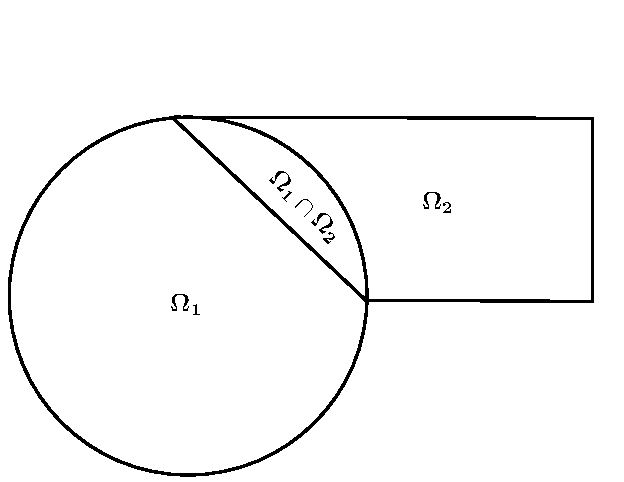
\includegraphics[width=.40\linewidth]{dd2dgeometry.pdf}}
  \hspace{0.25cm}
  \subfigure[Two overlapping meshes]{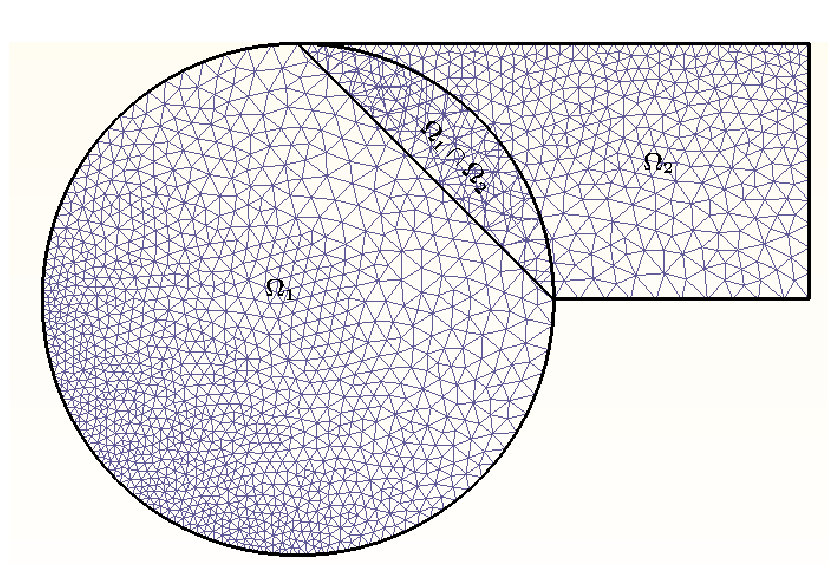
\includegraphics[width=.38\linewidth]{dd2dmesh.pdf}}
  \caption{geometry}
  \label{fig:original}
\end{figure}

\vspace{0.3cm}
\begin{center}
  \begin{tabular}{|c|c|c|}
  \hline
   \textbf{Nomber of iterations} & $\mathbf {\| u_1-u_{ex}\|_{L_2} }$ & $\mathbf{\| u_2-u_{ex}\|_{L_2}}$ \\
   \hline
    11 & 2.52e-8 & 2.16e-8 \\
   \hline
 \end{tabular}
\end{center}
% \begin{center}
% \begin{tabular}{|c|c|c|c|}
%   \hline
%   \textbf{Overlap} & \textbf{Nomber of iterations} & $\mathbf {\| u_1-u_{ex}\|_{L_2} }$ & $\mathbf{\| u_2-u_{ex}\|_{L_2}}$ \\
%   \hline
%    0 & -  & - & - \\
%   \hline
%   0.25 & 11 & 2.52e-8 & 2.16e-8 \\
%   \hline
%   0.50 & 8 & 2.34e-8 & 2.34e-8 \\
%   \hline
%   0.75 & 5 & 2.16e-8 & 2.31e-8 \\
%   \hline
%   1 & 2 & 2.11e-8 & 2.09e-8 \\
%   \hline
% \end{tabular}
% \end{center}
\vspace{0.2cm}
\subsection{Numerical solutions in 2D case}
\label{sec:numerical-solutions}
%$\Big \Omega_1$
% \begin{figure}[htbp]
% \centering
% \includegraphics[width=.5\linewidth]{dd2d.pdf}
%   \caption{The two overlapping meshes }
%   \label{fig:14}
% \end{figure}
\begin{figure}[htbp]
  \centering
  \subfigure[first iteration]{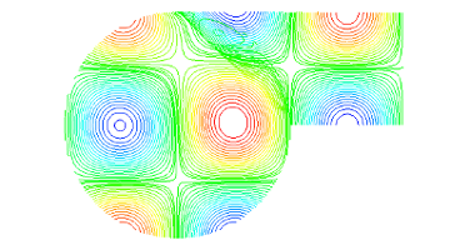
\includegraphics[width=.48\linewidth]{iter_1.png}}
  \subfigure[$10^{th}$ iteration]{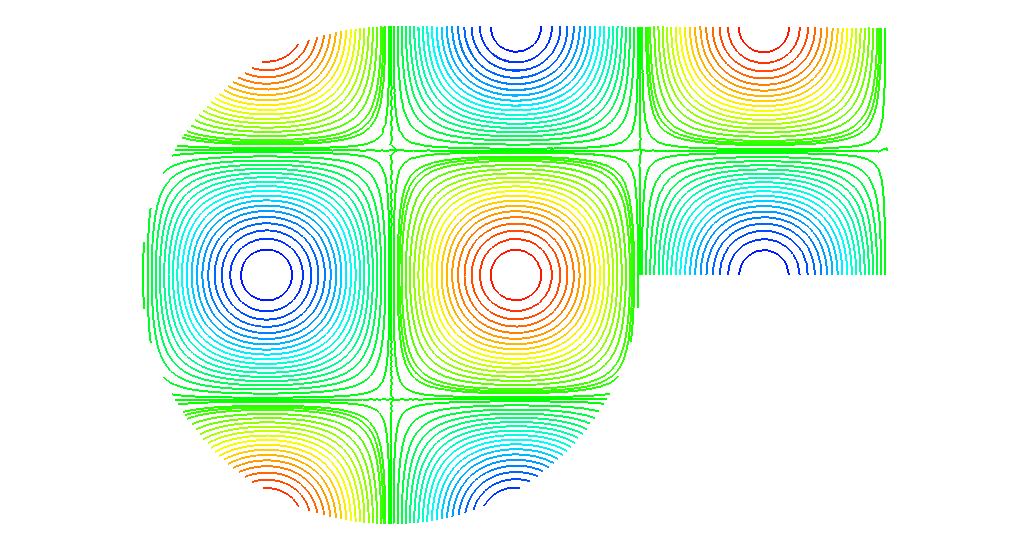
\includegraphics[width=.48\linewidth]{iter_10.png}}
  \caption{isovalues of solution in 2D}
  \label{fig:original}
\end{figure}


\section{Computing the eigenmodes of the Dirichlet to Neumann operator}
\label{sec:comp-eigenm-dirichl}

\subsection{Problem description and variational formulation}
\label{sec:probl-descr-vari}

We consider at the continuous level the Dirichlet-to-Neumann(DtN) map on $\Omega$, denoted by DtN$_{\Omega}$.

Let $u: \Gamma \longmapsto \mathbb R, $
\begin{equation*}
  \label{eq:35}
\text{DtN}_{\Omega}(u) = \kappa \frac{\partial v}{ n} \Big |_{\Gamma}
\end{equation*}
where $v$ satisfies
\begin{equation}
  \label{eq:36}
\left\{
  \begin{aligned}
    & \mathcal L(v):= (\eta - \text{div}(\kappa \nabla))v = 0 & \text{dans} \quad \Omega,\\
    & v = u & \text{sur} \quad \Gamma
  \end{aligned}
\right.
\end{equation}

where $\Omega$ is a bounded domain of $\mathbb R^d$ (d=2 or 3), and $\Gamma$ it border, $\kappa$ is a positive
diffusion function which can be discontinuous, and $\eta \geq 0$. The eigenmodes of the Dirichlet-to-Neumann
operator are solutions of the following eigenvalues problem
\begin{equation}
  \label{eq:37}
  \text{DtN}_{\Omega}(u) = \lambda \kappa u
\end{equation}
To obtain the discrete form of the DtN map, we consider the variational form of (\ref{eq:36}). let's define the
bilinear form $a~:~H^1(\Omega) \times H^1(\Omega) \longrightarrow \mathbb R $,
\begin{equation*}
  \label{eq:41}
  a(w,v) := \int_\Omega \eta w v + \kappa \nabla w \cdot \nabla v .
\end{equation*}
With a finite element basis $\{ \phi_k \}$, the coefficient matrix of a Neumann boundary value problem in $\Omega$ is
\begin{equation*}
\label{eq:42}
  A_{kl} := \int_\Omega \eta \phi_k \phi_l + \kappa \nabla \phi_k \cdot \nabla \phi_l .
\end{equation*}
A variational formulation of the flux reads
\begin{equation*}
  \label{eq:43}
\int_\Gamma \kappa \dfrac{\partial v}{\partial n} \phi_k = \int_\Omega \eta v \phi_k + \kappa \nabla v \cdot \nabla \phi_k \quad \forall~ \phi_k.
\end{equation*}
So the variational formulation of the eigenvalue problem (\ref{eq:37}) reads
\begin{equation}
\label{eq:40}
 \int_\Omega \eta v \phi_k + \kappa \nabla v \cdot \nabla \phi_k = \lambda \int_\Gamma \kappa v \phi_k  \quad \forall~ \phi_k.
\end{equation}
Let $B$ be the weighted mass matrix
\begin{equation*}
  \label{eq:44}
  (B)_{kl} = \int_\Gamma \kappa \phi_k \phi_l
\end{equation*}
The compact form of (\ref{eq:40}) is
\begin{equation}
  \label{eq:45}
  Av = \lambda B v
\end{equation}

\subsubsection{\FEEL implementation}
\label{sec:feel-implementation-1}

\begin{lstlisting}

// Assembly of the right hand side $ B = \mathlarger \int_\Gamma \kappa v w $
 auto B = M_backend->newMatrix( Xh, Xh ) ;
 form2( _test=Xh, _trial=Xh, _matrix=B, _init=true );
 BOOST_FOREACH( int marker, flags )
 {
   form2( Xh, Xh, B ) +=
   integrate( markedfaces(mesh,marker), kappa*idt(u)*id(v) );
 }
 B->close();
// Assembly of the left hand side $ A = \mathlarger \int_\Omega \eta v w + \kappa \nabla v \cdot \nabla w $
 auto A = M_backend->newMatrix( Xh, Xh ) ;
 form2( _test=Xh, _trial=Xh, _matrix=A, _init=true ) =
 integrate( elements(mesh), kappa*gradt(u)*trans(grad(v)) + nu*idt(u)*id(v) );
 A->close();

// eigenvalue solver options
 int nev = this->vm()["solvereigen-nev"].template as<int>();
 int ncv = this->vm()["solvereigen-ncv"].template as<int>();;
// definition of the eigenmodes
 SolverEigen<double>::eigenmodes_type modes;
// solve the eigenvalue problem $ Av =  \lambda B v $
 modes=
       eigs( _matrixA=A,
             _matrixB=B,
             _nev=nev,
             _ncv=ncv,
             _transform=SINVERT,
             _spectrum=SMALLEST_MAGNITUDE,
             _verbose = true );

}

\end{lstlisting}

\subsection{Numerical solutions}
\label{sec:numerical-solutions-1}
\vspace{-17pt}
\begin{figure}[htbp]
  \centering
  \subfigure[first mode]{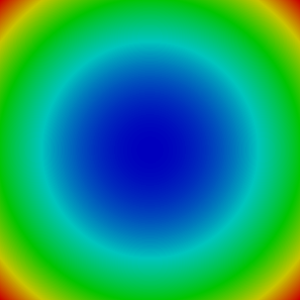
\includegraphics[width=.24\linewidth]{mode-0}}
  \hspace{0.3cm}
  \subfigure[second mode]{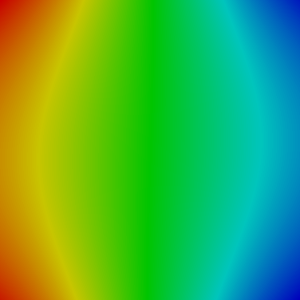
\includegraphics[width=.24\linewidth]{mode-1}}
  \hspace{0.3cm}
  \subfigure[third mode]{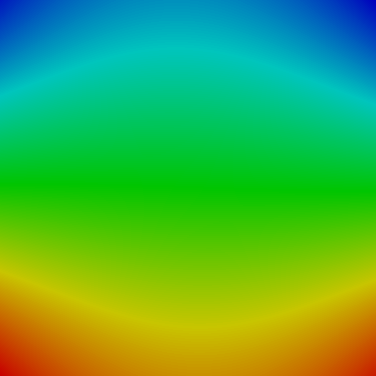
\includegraphics[width=.24\linewidth]{mode-2}}
  \caption{three eigenmodes}
\label{fig:eigenvalues}
\end{figure}
These numerical solutions correspond to the following configuration :
\begin{enumerate}
\item $\mathbb P_2$ approximation~:~ the lagrange polynomial order
\item hsize $= 0.02$~:~ the mesh size
\item $\mu = \kappa = 1.$
\end{enumerate}
%%% Local Variables:
%%% coding: utf-8
%%% mode: latex
%%% TeX-PDF-mode: t
%%% TeX-parse-self: t
%%% x-symbol-8bits: nil
%%% TeX-auto-regexp-list: TeX-auto-full-regexp-list
%%% TeX-master: "../feel-manual"
%%% ispell-local-dictionary: "american"
%%% End:
